\documentclass[11pt,a4paper]{article}
\usepackage{graphicx}
\usepackage{amsmath}
\usepackage{amssymb}
\usepackage{mathrsfs}
\usepackage{cancel}

\begin{document}
\begin{center}
\textbf{REPORTE DE TAREA}\\
EXPLICACION DE ARREGLOS Y PARAMETROS DE LOS AMPLIFICADORES CLASE B
\end{center}

\begin{center}
Maria de Lourdes Gomez Islas\\
08-OCT-2019\\
Universidad Politecnica de La Zona Metropolitana de Guadalajara
\end{center}

\part{Que es un amplificador clase B}
\textbf{Los amplificadores de clase B} se caracterizan por tener intensidad casi nula a través de sus transistores cuando no hay señal en la entrada del circuito, por lo que en reposo el consumo es casi nulo.\\
 Se les denomina amplificador clase B, cuando el voltaje de polarización y la máxima amplitud de la señal entrante poseen valores que hacen que la corriente de salida circule durante el semiciclo de la señal de entrada.\\
La característica principal de este tipo de amplificadores es el alto factor de amplificación. 

\begin{figure}[h]
\centering
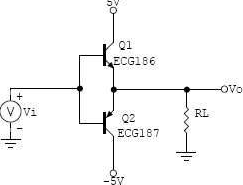
\includegraphics[width=8cm]{amplificadorclaseB.png} 
\caption{Amplificador clase B}
\end{figure}

\section{Ventajas}
\begin{itemize}
\item Posee bajo consumo en reposo.
\item Aprovecha al máximo la Corriente entregada por la fuente.
\item Intensidad casi nula cuando está en reposo.
\end{itemize}

\section{Desventajas}
\begin{itemize}
\item Producen armónicos, y es mayor cuando no tienen los transistores de salida con las mismas características técnicas, debido a esto se les suele polarizar de forma que se les introduce una pequeña polarización directa. Con esto se consigue desplazar las curvas y se disminuye dicha distorsión.
\end{itemize}

\part{Parametros de un amplificador Clase B}

Para la operacion de Clase B, se utilizan dos transistores de conmutacion complementarios con el punto Q (que es su punto de polarizacion) de cada transistor ubicado en su punto de corte.\\
Esto permite que un transistor amplifique la señal mas de la mitad de la forma de onda de entrada, mientras que el otro transistor amplifica la otra mitad.\\
Estas dos mitades amplificadas se combinan juntas en la carga para producir un ciclo completo de forma de onda. Este par complementario NPN-PNP tambien se conoce como una configuracion \textbf{push-pull}.\\
Debido a la polarizacion de corte, la corriente de reposo es cero cuando no hay señal de entrada, por lo tanto, no se disipa ni desperdicia potencia cuando los transistores estan en reposo, aumentando la eficiencia general de un amplificador de \textbf{Clase B} con respecto a la \textbf{Clase A.}

\part{Restricciones}

Sin embargo, como el amplificador de clase B esta polarizado de manera que la corriente de salida fluya a traves de cada transistor solo la mitad del ciclo de entrada, la forma de onda de salida no es una replica exacta de la forma de onda de entrada ya que la senal de salida esta distorsionada. Esta distorsion ocurre en cada cruce por cero de la senal de entrada produciendo lo que generalmente se llama distorsion cruzada cuando los dos transistores se "\textbf{ponen en ON}" entre si.\\
Este problema de distorsion puede superarse facilmente ubicando el punto de polarización del transistor ligeramente por encima del corte.\\
Al polarizar el transistor ligeramente por encima de su punto de corte pero muy por debajo del punto Q central del amplificador de \textbf{clase A}, podemos crear un circuito amplificador de \textbf{clase AB}. Entonces, el objetivo basico de un amplificador de clase AB es preservar la configuración basica de clase B, mientras que al mismo tiempo mejora su linealidad polarizando cada transistor de conmutacion ligeramente por encima del umbral.

\end{document}